\title{AI High-Performance Solution on FPGA}

\team{Nico Canzani, Dominik M\"uller}

% \client{FHNW Institute for Sensors and Electronics}
\client{Inst. for Sensors and Electronics}
% \client{FHNW / ISE}

\coaches{%
  Prof. Michael Pichler,\\
  Prof. Dr. Hanspeter Schmid
}

\repo{https://git.io/p5-aionfpga}
% curl -i https://git.io -F "url=https://github.com/MuellerDominik/P5-AIonFPGA/" -F "code=p5-aionfpga"

\fssummary{
  In a world of self-driving cars and automated quality control in manufacturing, real-time image classification is becoming increasingly important.
  % Artificial intelligence, and deep learning in particular, are achieving excellent classification accuracies, but there are some challenges.
  Artificial intelligence (AI), and deep learning in particular, are achieving excellent classification accuracies.
  % However, a large labeled dataset of training data is required to train deep convolutional neural networks.
  % However, a large labeled dataset of training data is required to train a convolutional neural networks (CNN).
  However, the training of a convolutional neural network (CNN) requires a sufficiently large labeled dataset.
  % However, the training of a deep convolutional neural network (CNN) required a sufficiently large labeled dataset.
}

\fsgraphics{
  \begin{minipage}[t]{0.5\textwidth}
      \begin{minipage}[t]{0.98\textwidth}
        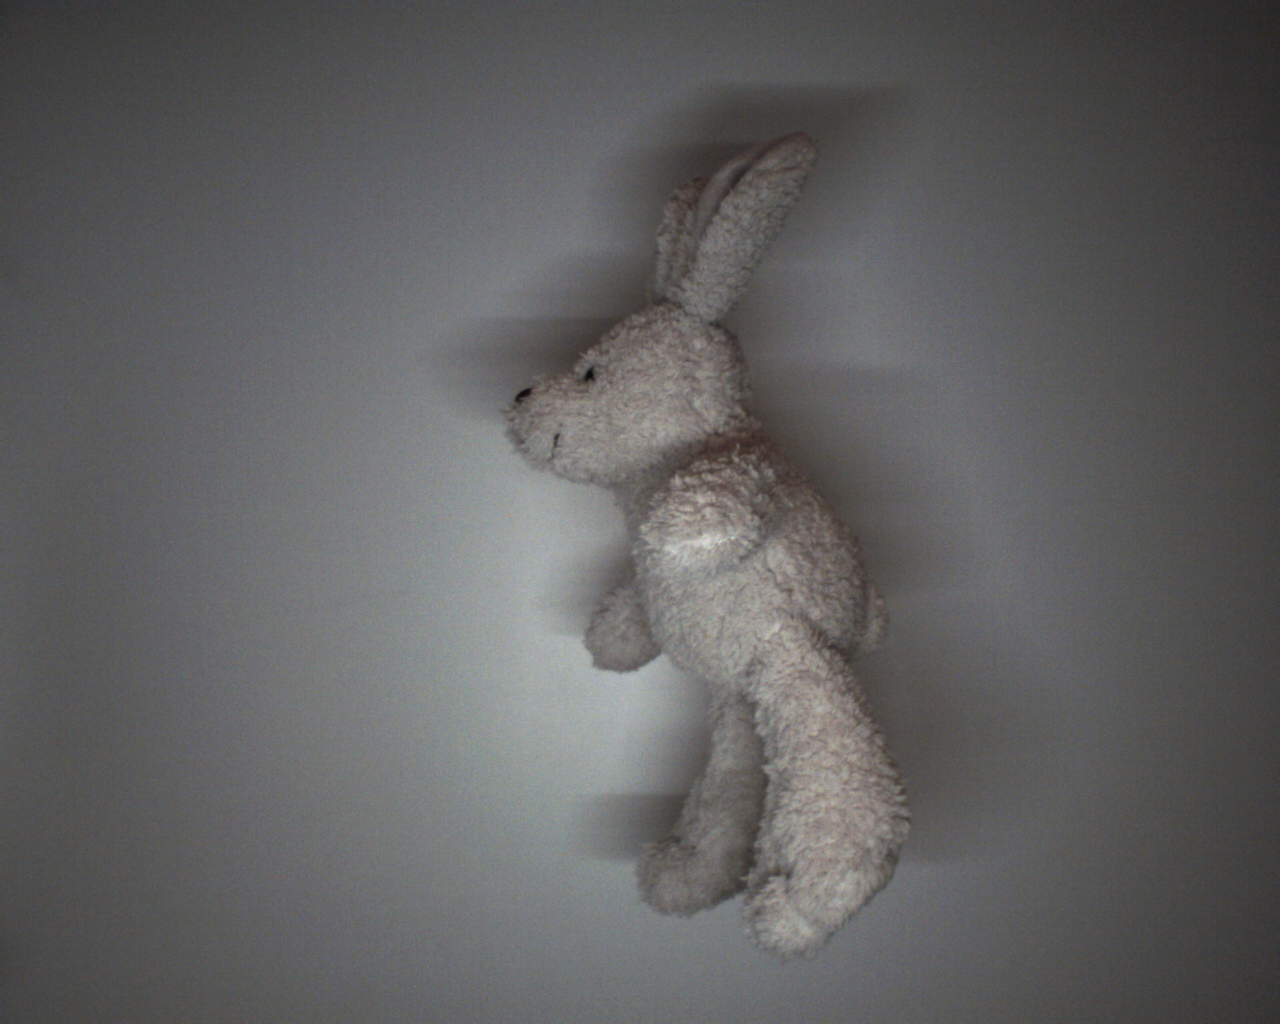
\includegraphics[width=\textwidth]{graphics/1574952009_278_10_stuffed-bunny.png}
        \graphicscaption{Image of the \textit{Stuffed Bunny}} % Example / Sample
      \end{minipage}
  \end{minipage}%
  \begin{minipage}[t]{0.5\textwidth}
    \begin{flushright}
      \begin{minipage}[t]{0.98\textwidth}
        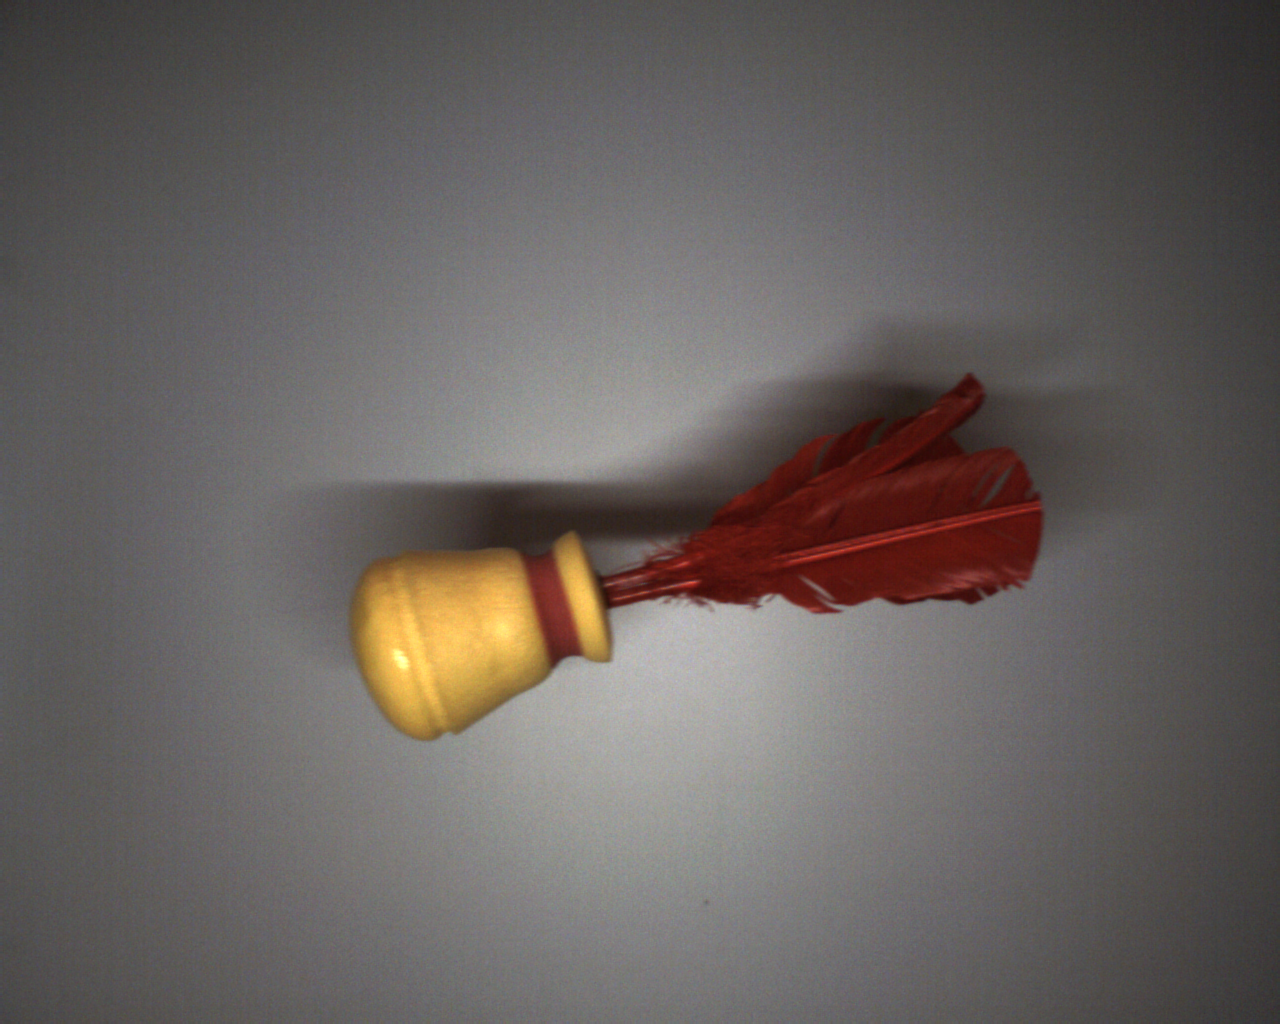
\includegraphics[width=\textwidth]{graphics/1574943825_125_8_hand-featherball.png}
        \graphicscaption{Image of the \textit{Hand Featherball}} % Example / Sample
      \end{minipage}
    \end{flushright}
  \end{minipage}
}

\fscontent{
  % \section{Problem Statement}
  \section{Difficulty}
  Collecting a sufficiently large dataset of pictures is not trivial.
  When done manually, the camera has to be started and stopped for each throw.
  This likely creates many empty frames at the beginning and at the end of the capture.
  Those empty and therefore invalid frames must be removed to avoid errors during the training of the CNN later on.
  Furthermore, each valid frame must be labeled.
  This procedure is very error-prone if it is performed manually for each individual frame.

  \newcol
  \section{Software}
  % To reliably detect a throw, a simple image change detection algorithm is implemented.
  % It requires a repeated difference computation and therefore a circular buffer is used.
  % To simplify this task, a camera throw detection mechanism is implemented and various Python scripts are used.
  To simplify the image collection, a camera throw detection mechanism is implemented and various Python scripts are used.
  The goal of the throw detection is to extract valid frames of a throw --- with objects on them --- from the continuous data stream of the camera.
  Therefore, the throw detection needs to work in real time.
  % At a frame rate of \SI{200}{fps}, there is $<\SI{5}{ms}$ to process a single frame (without the use of parallel computing).
  At a frame rate of \SI{200}{fps}, there is less than \SI{5}{ms} to process a single frame.
  % Due to this time constraint, a simple image change detection algorithm is employed.
  Due to this time constraint, a simple image change detection algorithm is implemented.

  \newcol
  % \section{Labeled Dataset}
  \section{Dataset}
  % The dataset contains images of 22 different throwing objects.
  The dataset contains images of 22 different throwing objects, ranging from sports equipment to toys.
  It is fully labeled and consists of more than \num{15000} usable images with at least 480 images of each object.
  % All images were collected over the course of two days.
  % The employed software allowed to collected all images over the course of two days.
  The employed software made it possible to collect all images over the course of only two days.
  % The above images show an example image of the \textit{Stuffed Bunny} and of the \textit{Hand Featherball}.
  The above images are two examples from the labeled dataset.
  The first one shows the \textit{Stuffed Bunny} and the second one shows the \textit{Hand Featherball}.
}

\infobox{Throwing Booth}{
  % \begin{minipage}[t][][b]{0.45\textwidth}
  %   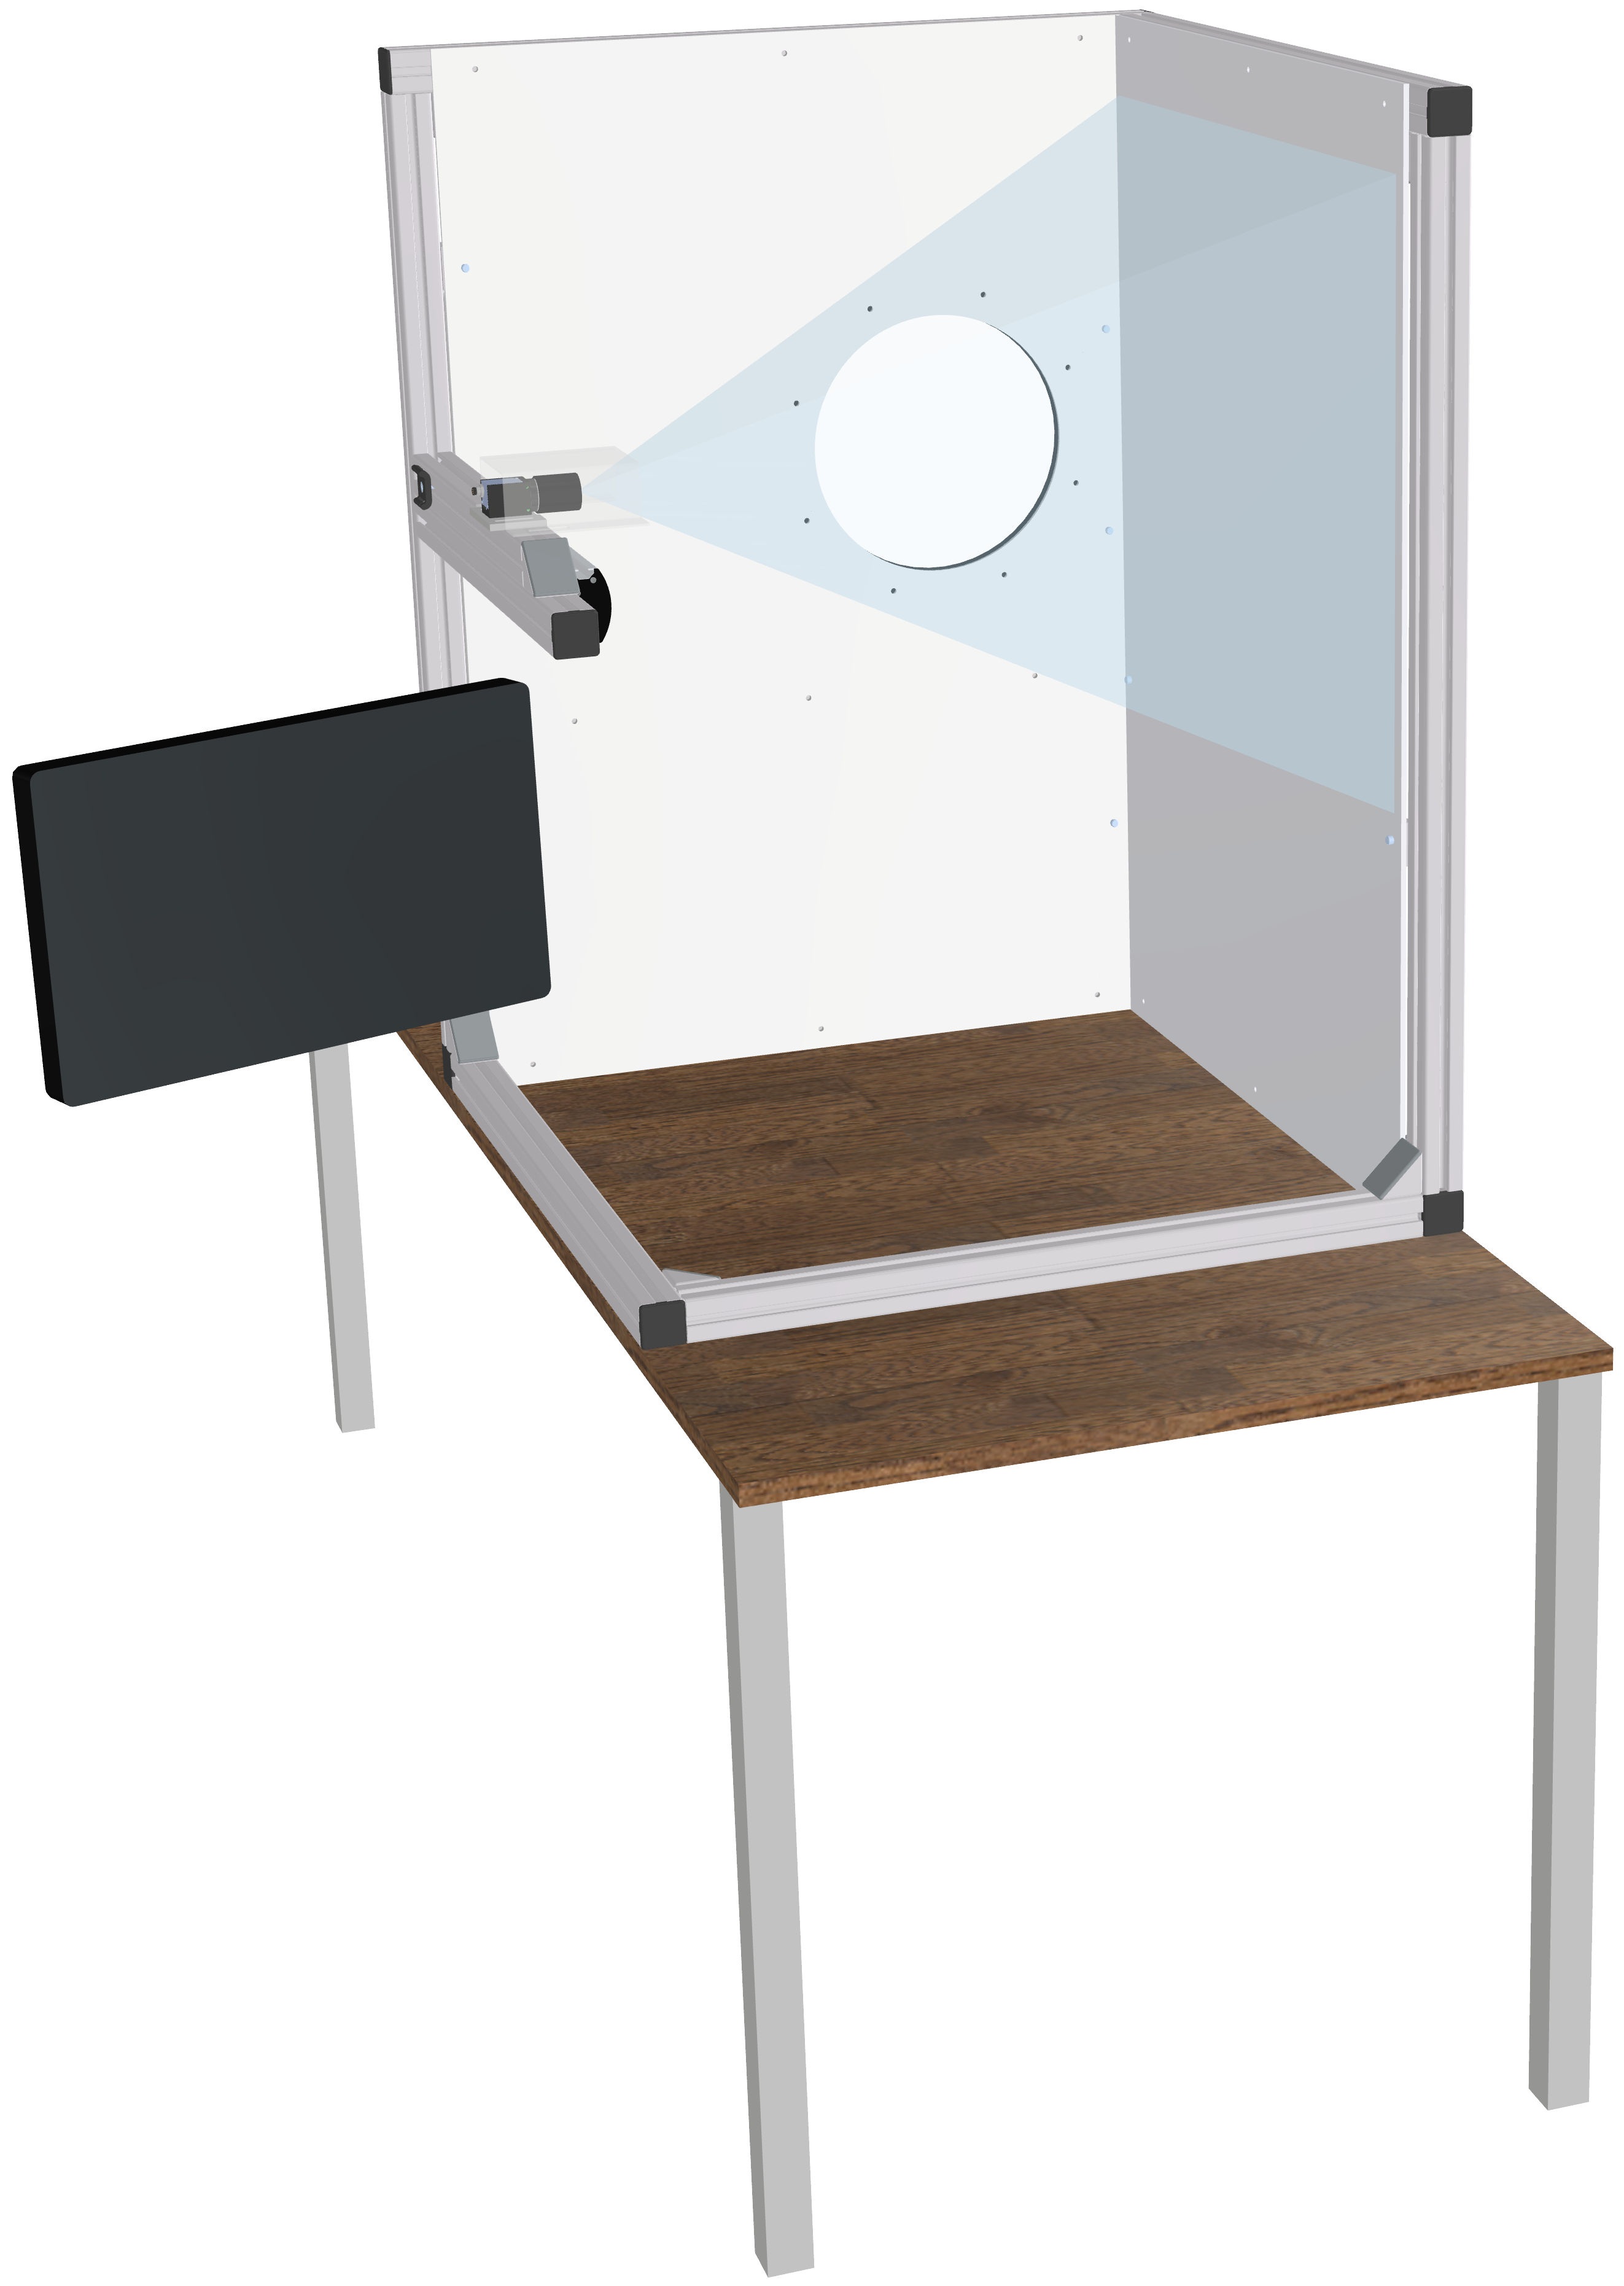
\includegraphics[height=50mm]{graphics/top_assembly.png}
  % \end{minipage}\hfill%
  \begin{minipage}{0.65\textwidth}
    The throwing booth is constructed from general-purpose aluminium profiles.
    % The rear panel is made of a white ABS plastic sheet for its robust impact strength and has a target hole. % features a target hole
    Due to its robust impact strength, the rear panel is made of a white ABS plastic sheet and has a target hole.
    % The side panel is made of a foamed PVC sheet to reduce light reflections.
    The white side panel serves as a consistent background for the images.
    It is made of a foamed PVC sheet with a fine-textured surface to reduce light reflections.
    % The image acquisition system consists of a Baumer industrial camera and a suitable lens.
    The image acquisition system consists of a Baumer industrial camera combined with a suitable lens. % imaging environment
    % Strong diffuse lighting is used to minimize the required exposure time and to evenly illuminate the side panel.
    Strong diffuse lighting is used to minimize the required exposure time and to illuminate the side panel as evenly as possible.
    % A monitor is used to display the detected object. % display the result
    Finally, a monitor is used to display the detected object.
  \end{minipage}\hfill%
  \begin{minipage}{0.32\textwidth}
    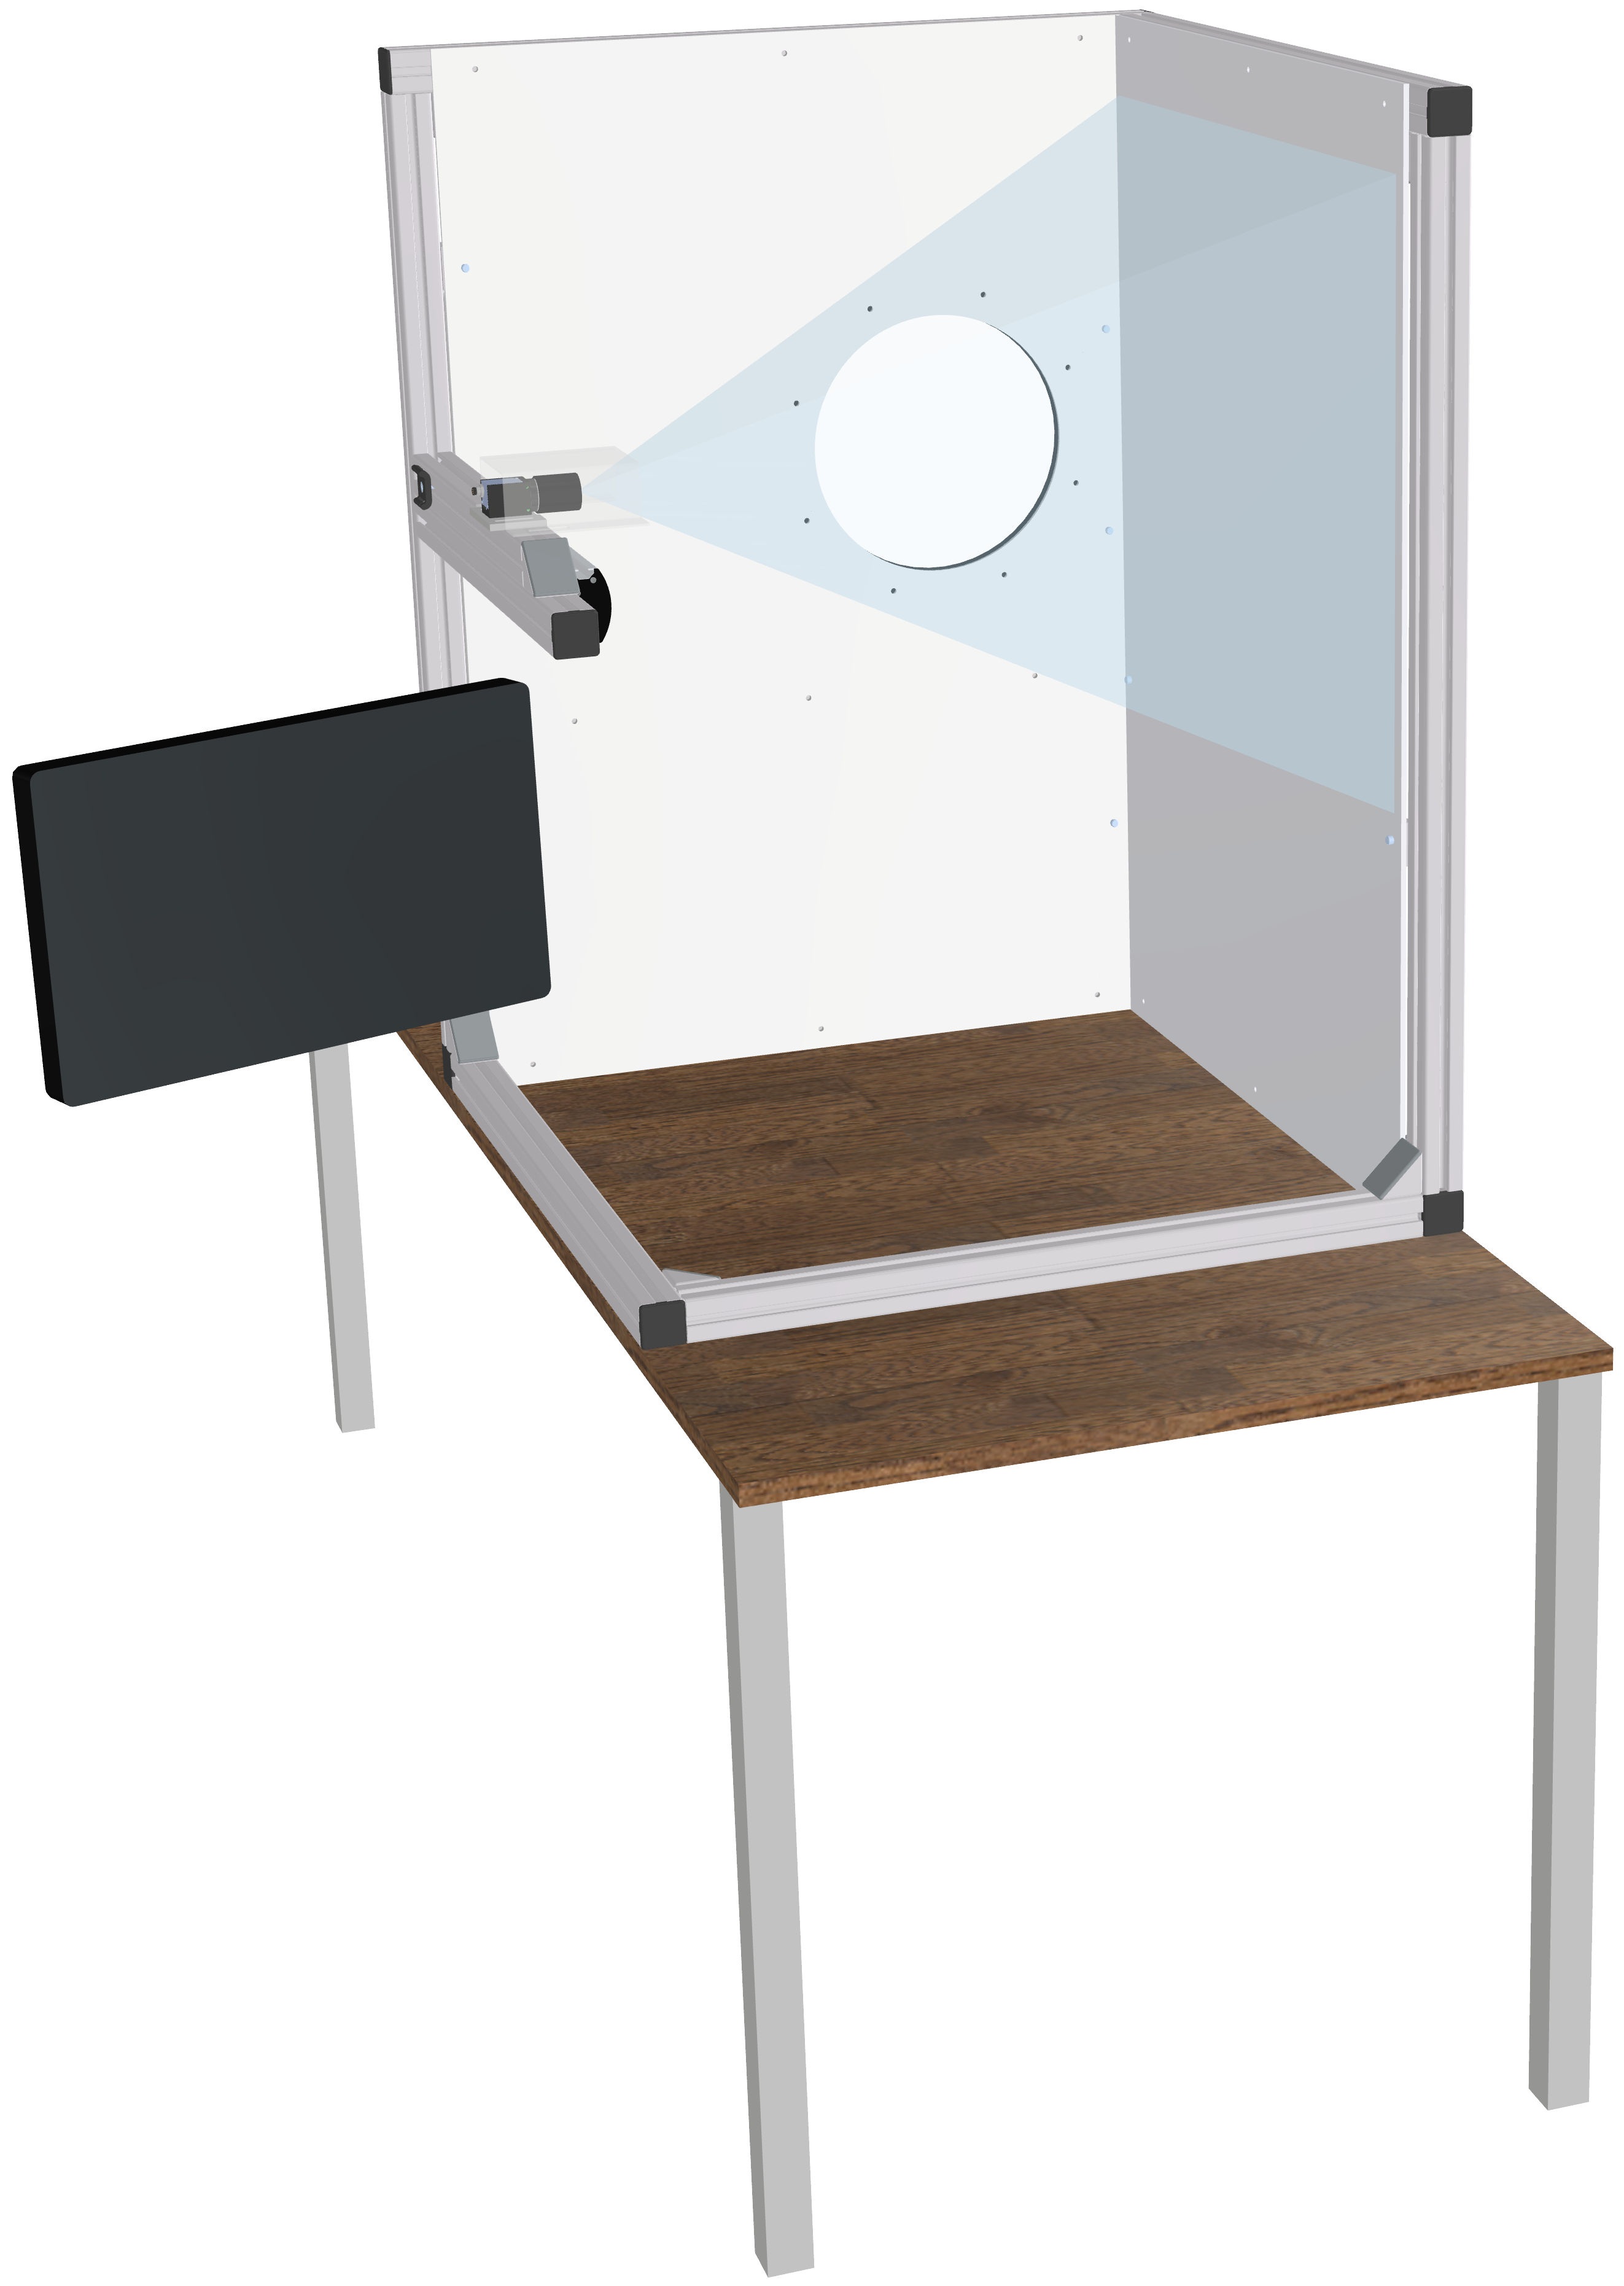
\includegraphics[width=\textwidth]{graphics/top_assembly.png}
  \end{minipage}
}
